% Name: Mind map
% Description: A thesis plan with four colored branches, each with two sub-topics.
% Tags: mind map, planning, brainstorming

\usetikzlibrary{mindmap}

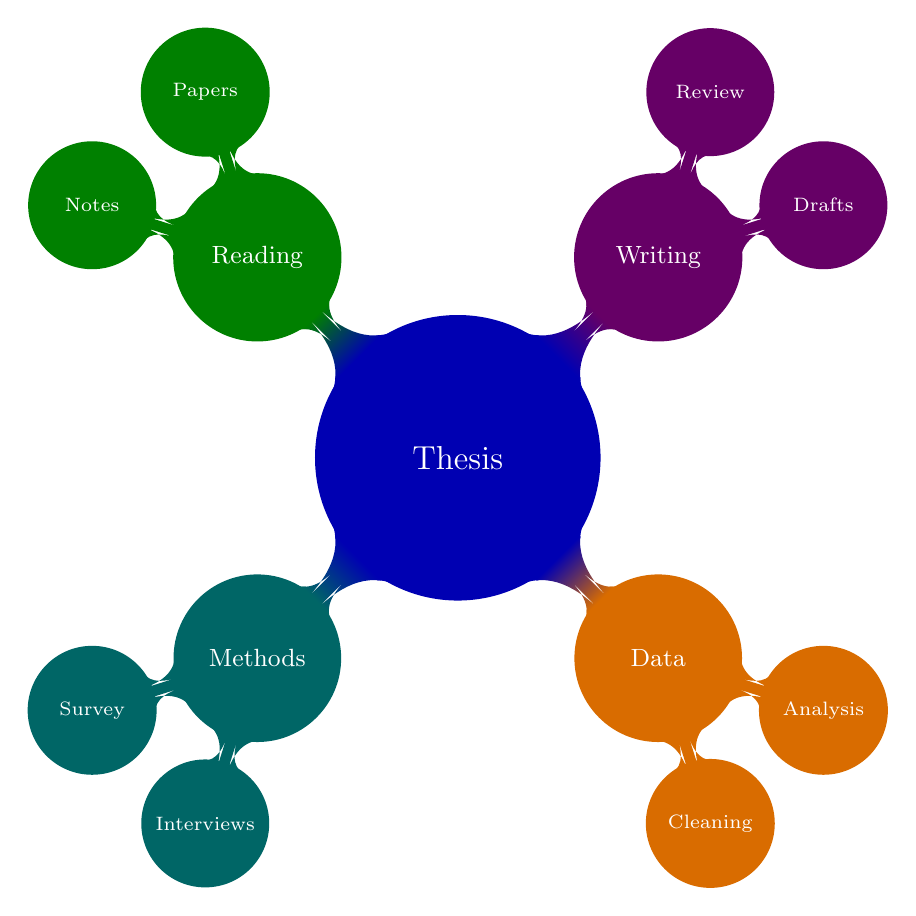
\begin{tikzpicture}[
  mindmap, grow cyclic,
  every node/.style={concept, execute at begin node=\hskip0pt},
  concept color=blue!70!black, text=white,
  root concept/.append style={minimum size=26mm, font=\large},
  level 1/.append style={level distance=36mm, sibling angle=90, minimum size=18mm, font=\small},
  level 2/.append style={level distance=22mm, sibling angle=55, minimum size=14mm, font=\scriptsize},
]
  \node[root concept] {Thesis}
    child[concept color=teal!80!black] { node {Methods}
      child { node {Survey} }
      child { node {Interviews} }
    }
    child[concept color=orange!85!black] { node {Data}
      child { node {Cleaning} }
      child { node {Analysis} }
    }
    child[concept color=violet!80!black] { node {Writing}
      child { node {Drafts} }
      child { node {Review} }
    }
    child[concept color=green!50!black] { node {Reading}
      child { node {Papers} }
      child { node {Notes} }
    };
\end{tikzpicture}
